% Created by tikzDevice version 0.7.0 on 2015-04-23 17:27:43
% !TEX encoding = UTF-8 Unicode
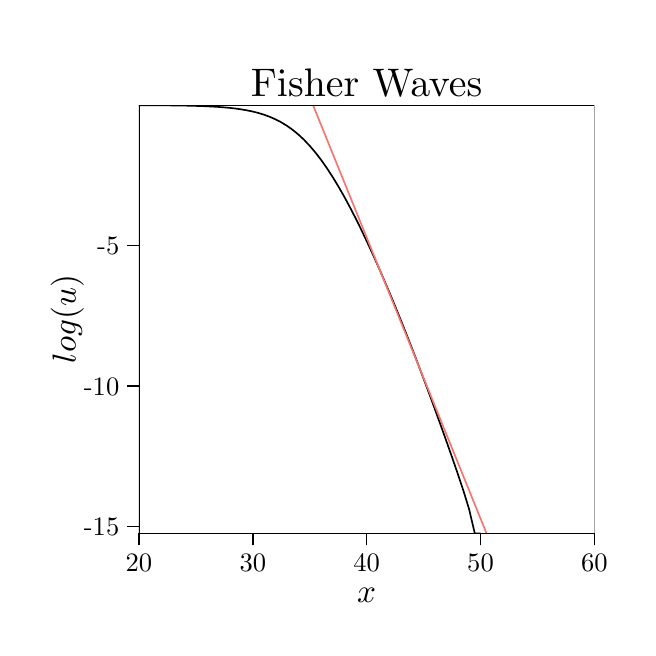
\begin{tikzpicture}[x=1pt,y=1pt]
\definecolor[named]{fillColor}{rgb}{1.00,1.00,1.00}
\path[use as bounding box,fill=fillColor,fill opacity=0.00] (0,0) rectangle (216.81,216.81);
\begin{scope}
\path[clip] (  0.00,  0.00) rectangle (216.81,216.81);
\definecolor[named]{drawColor}{rgb}{1.00,1.00,1.00}
\definecolor[named]{fillColor}{rgb}{1.00,1.00,1.00}

\path[draw=drawColor,line width= 0.6pt,line join=round,line cap=round,fill=fillColor] (  0.00,  0.00) rectangle (216.81,216.81);
\end{scope}
\begin{scope}
\path[clip] ( 40.22, 34.03) rectangle (204.76,188.82);
\definecolor[named]{fillColor}{rgb}{1.00,1.00,1.00}

\path[fill=fillColor] ( 40.22, 34.03) rectangle (204.76,188.82);
\definecolor[named]{drawColor}{rgb}{0.00,0.00,0.00}

\path[draw=drawColor,line width= 0.6pt,line join=round] ( 40.22,188.79) --
	( 42.28,188.78) --
	( 44.33,188.77) --
	( 46.39,188.76) --
	( 48.45,188.75) --
	( 50.50,188.73) --
	( 52.56,188.70) --
	( 54.62,188.68) --
	( 56.67,188.64) --
	( 58.73,188.60) --
	( 60.79,188.54) --
	( 62.84,188.47) --
	( 64.90,188.39) --
	( 66.96,188.28) --
	( 69.02,188.16) --
	( 71.07,188.00) --
	( 73.13,187.81) --
	( 75.19,187.57) --
	( 77.24,187.28) --
	( 79.30,186.92) --
	( 81.36,186.49) --
	( 83.41,185.97) --
	( 85.47,185.34) --
	( 87.53,184.58) --
	( 89.58,183.67) --
	( 91.64,182.60) --
	( 93.70,181.35) --
	( 95.75,179.89) --
	( 97.81,178.20) --
	( 99.87,176.28) --
	(101.92,174.11) --
	(103.98,171.69) --
	(106.04,169.02) --
	(108.09,166.10) --
	(110.15,162.94) --
	(112.21,159.55) --
	(114.27,155.96) --
	(116.32,152.16) --
	(118.38,148.18) --
	(120.44,144.02) --
	(122.49,139.71) --
	(124.55,135.26) --
	(126.61,130.67) --
	(128.66,125.95) --
	(130.72,121.12) --
	(132.78,116.18) --
	(134.83,111.13) --
	(136.89,105.98) --
	(138.95,100.74) --
	(141.00, 95.40) --
	(143.06, 89.98) --
	(145.12, 84.47) --
	(147.17, 78.88) --
	(149.23, 73.20) --
	(151.29, 67.44) --
	(153.34, 61.60) --
	(155.40, 55.64) --
	(157.46, 49.48) --
	(159.52, 42.77) --
	(161.57, 34.03) --
	(163.63, 34.03);
\definecolor[named]{drawColor}{rgb}{0.97,0.46,0.43}
\definecolor[named]{fillColor}{rgb}{0.97,0.46,0.43}

\path[draw=drawColor,line width= 0.6pt,line join=round,fill=fillColor] ( 91.78,216.81) -- (179.61,  0.00);
\definecolor[named]{drawColor}{rgb}{0.00,0.00,0.00}

\path[draw=drawColor,line width= 0.6pt,line join=round,line cap=round] ( 40.22, 34.03) rectangle (204.76,188.82);
\end{scope}
\begin{scope}
\path[clip] (  0.00,  0.00) rectangle (216.81,216.81);
\definecolor[named]{drawColor}{rgb}{0.00,0.00,0.00}

\node[text=drawColor,anchor=base east,inner sep=0pt, outer sep=0pt, scale=  0.96] at ( 33.11, 33.19) {-15};

\node[text=drawColor,anchor=base east,inner sep=0pt, outer sep=0pt, scale=  0.96] at ( 33.11, 83.97) {-10};

\node[text=drawColor,anchor=base east,inner sep=0pt, outer sep=0pt, scale=  0.96] at ( 33.11,134.74) {-5};
\end{scope}
\begin{scope}
\path[clip] (  0.00,  0.00) rectangle (216.81,216.81);
\definecolor[named]{drawColor}{rgb}{0.00,0.00,0.00}

\path[draw=drawColor,line width= 0.6pt,line join=round] ( 35.95, 36.50) --
	( 40.22, 36.50);

\path[draw=drawColor,line width= 0.6pt,line join=round] ( 35.95, 87.27) --
	( 40.22, 87.27);

\path[draw=drawColor,line width= 0.6pt,line join=round] ( 35.95,138.05) --
	( 40.22,138.05);
\end{scope}
\begin{scope}
\path[clip] (  0.00,  0.00) rectangle (216.81,216.81);
\definecolor[named]{drawColor}{rgb}{0.00,0.00,0.00}

\path[draw=drawColor,line width= 0.6pt,line join=round] ( 40.22, 29.77) --
	( 40.22, 34.03);

\path[draw=drawColor,line width= 0.6pt,line join=round] ( 81.36, 29.77) --
	( 81.36, 34.03);

\path[draw=drawColor,line width= 0.6pt,line join=round] (122.49, 29.77) --
	(122.49, 34.03);

\path[draw=drawColor,line width= 0.6pt,line join=round] (163.63, 29.77) --
	(163.63, 34.03);

\path[draw=drawColor,line width= 0.6pt,line join=round] (204.76, 29.77) --
	(204.76, 34.03);
\end{scope}
\begin{scope}
\path[clip] (  0.00,  0.00) rectangle (216.81,216.81);
\definecolor[named]{drawColor}{rgb}{0.00,0.00,0.00}

\node[text=drawColor,anchor=base,inner sep=0pt, outer sep=0pt, scale=  0.96] at ( 40.22, 20.31) {20};

\node[text=drawColor,anchor=base,inner sep=0pt, outer sep=0pt, scale=  0.96] at ( 81.36, 20.31) {30};

\node[text=drawColor,anchor=base,inner sep=0pt, outer sep=0pt, scale=  0.96] at (122.49, 20.31) {40};

\node[text=drawColor,anchor=base,inner sep=0pt, outer sep=0pt, scale=  0.96] at (163.63, 20.31) {50};

\node[text=drawColor,anchor=base,inner sep=0pt, outer sep=0pt, scale=  0.96] at (204.76, 20.31) {60};
\end{scope}
\begin{scope}
\path[clip] (  0.00,  0.00) rectangle (216.81,216.81);
\definecolor[named]{drawColor}{rgb}{0.00,0.00,0.00}

\node[text=drawColor,anchor=base,inner sep=0pt, outer sep=0pt, scale=  1.20] at (122.49,  9.03) {$x$};
\end{scope}
\begin{scope}
\path[clip] (  0.00,  0.00) rectangle (216.81,216.81);
\definecolor[named]{drawColor}{rgb}{0.00,0.00,0.00}

\node[text=drawColor,rotate= 90.00,anchor=base,inner sep=0pt, outer sep=0pt, scale=  1.20] at ( 17.30,111.43) {$log(u)$};
\end{scope}
\begin{scope}
\path[clip] (  0.00,  0.00) rectangle (216.81,216.81);
\definecolor[named]{drawColor}{rgb}{0.00,0.00,0.00}

\node[text=drawColor,anchor=base,inner sep=0pt, outer sep=0pt, scale=  1.44] at (122.49,191.84) {Fisher Waves};
\end{scope}
\end{tikzpicture}
